% this file contains all the graphics for the paper
%
% I chose to do it this way because 
% it is easier to move graphics around within the paper
% instead of copy pasting entire figure definitions,
% it is necessary only to copy-paste the include tag
% shows the pressure density for one of our users

%
% solution graphics
%

%<*final>

% describes how the Markov model will look after it has been constructed
\begin{figure}
\centering
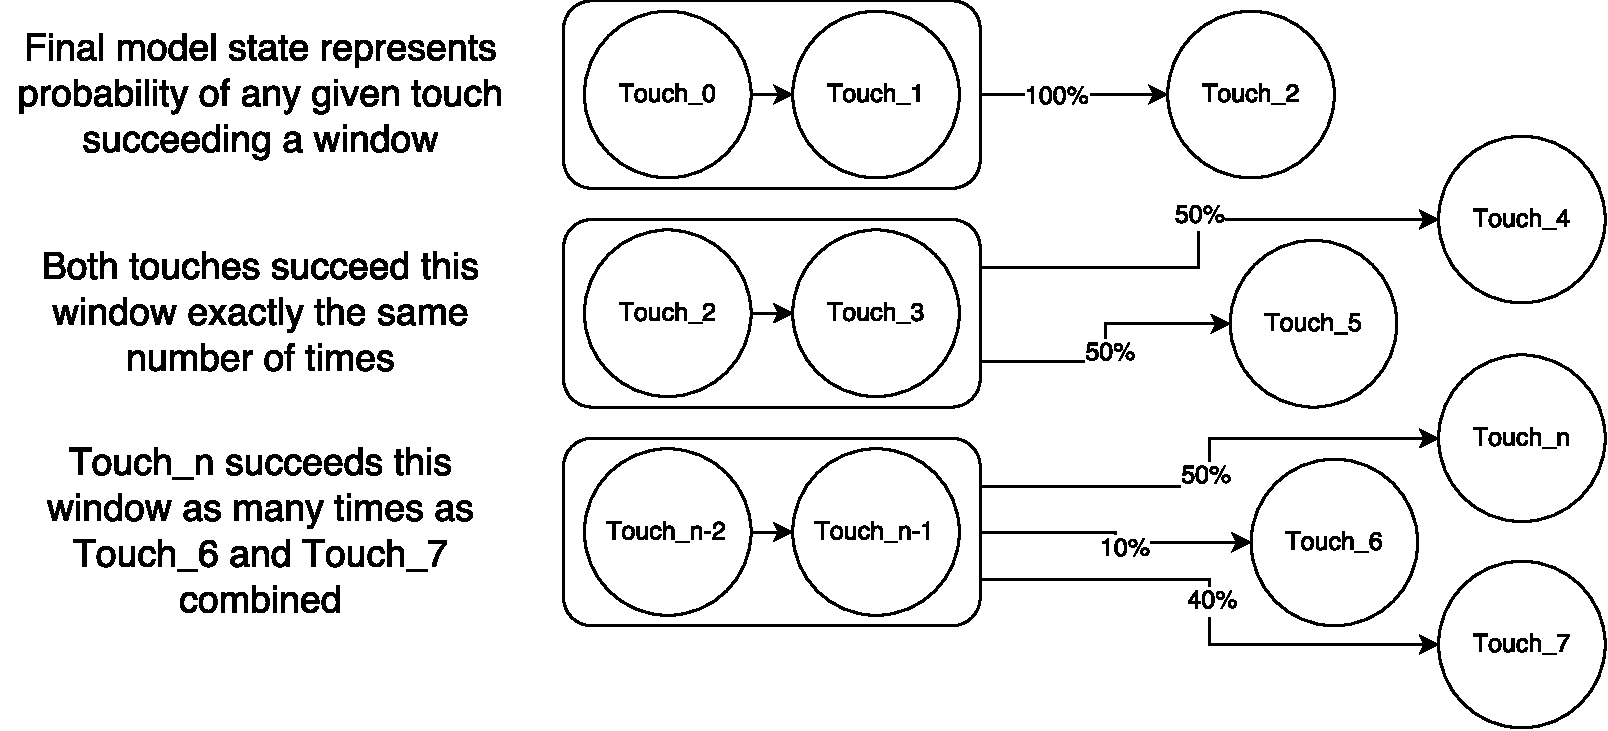
\includegraphics[width=.45\textwidth]{final_marcov_model_state.pdf}
\caption{
Example $2$-Markov model after the probabilities have been calculated.
The rounded rectangles indicate 
a sequence of touch interactions 
which precede the following touch interaction with some probability $p$.
$p$ for token $T$ after sequence $W$ is computed 
as occurrences of $T$ after $W$
by occurrences of $W$.
% The top window states that 
% Touch\_2 succeeds the sequence Touch\_0, Touch\_1 with probability $100$\%.
}
\label{fig:final_markov_model_state}
\end{figure}

%</final>

%<*token>

% show the range over which tokens are created
\begin{figure}
\centering
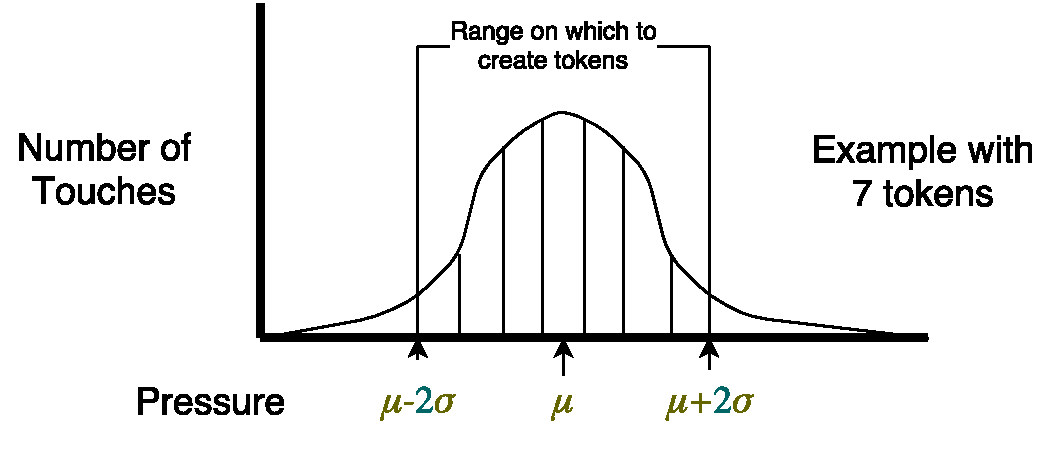
\includegraphics[width=.45\textwidth, keepaspectratio]{token_creation.pdf}
\caption{
Tokens are only created for 
pressure range $\mu \pm 2\sigma$ 
for each key.
Touches with pressure values
$p>\mu + 2\sigma$ and $p<\mu - 2\sigma$
are thrown out.
This eliminates outliers creating
increased reproducibility.
}
\label{fig:token_creation}
\end{figure}

%</token>

%<*phone>

% visually drive the process of token creation
% this shows a model with k=3
\begin{figure}
\centering
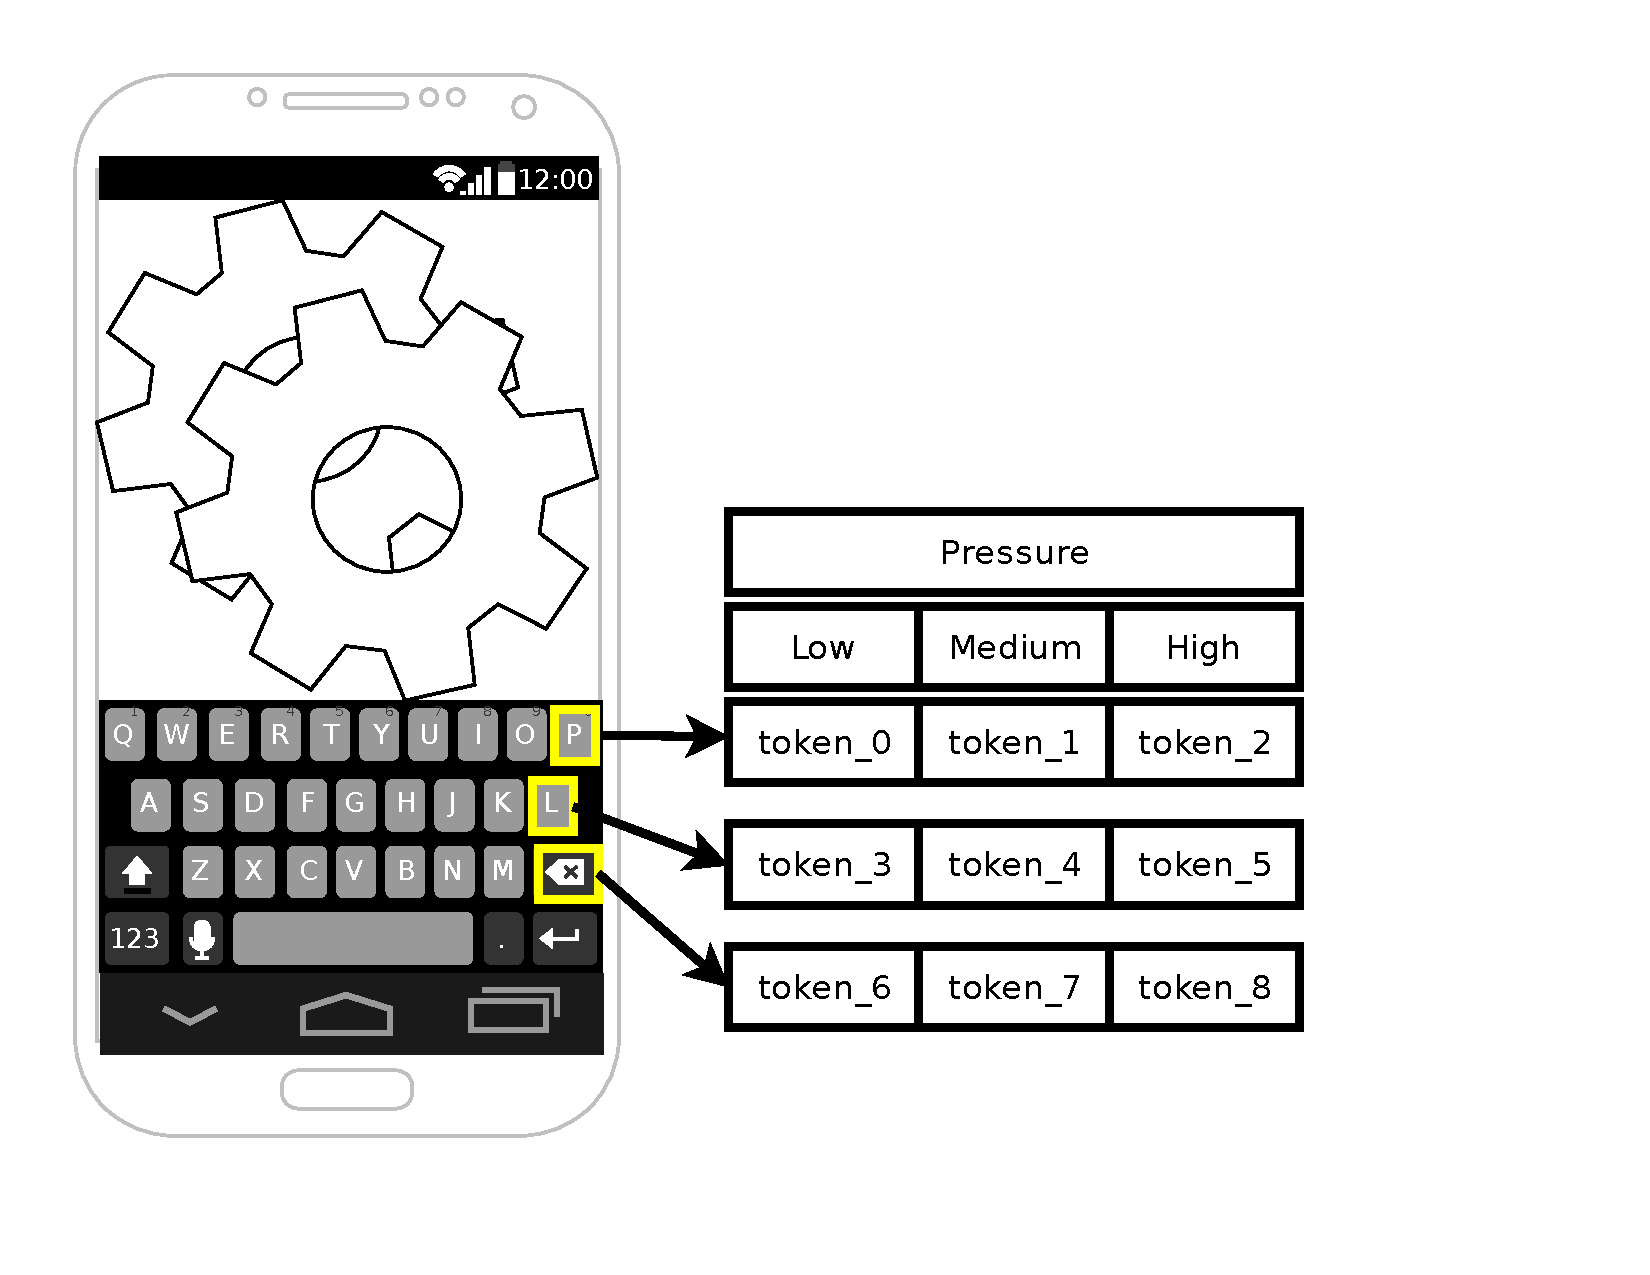
\includegraphics[width=.45\textwidth, keepaspectratio]{phone_tokens.pdf}
\caption{
Multiple tokens, $k=3$ above, correspond to each key location.
A touch screen interaction is assigned a token based on
key location and pressure.
}
\label{fig:phone_tokens}
\end{figure}

%</phone>

%<*markov>

\begin{figure}
\centering
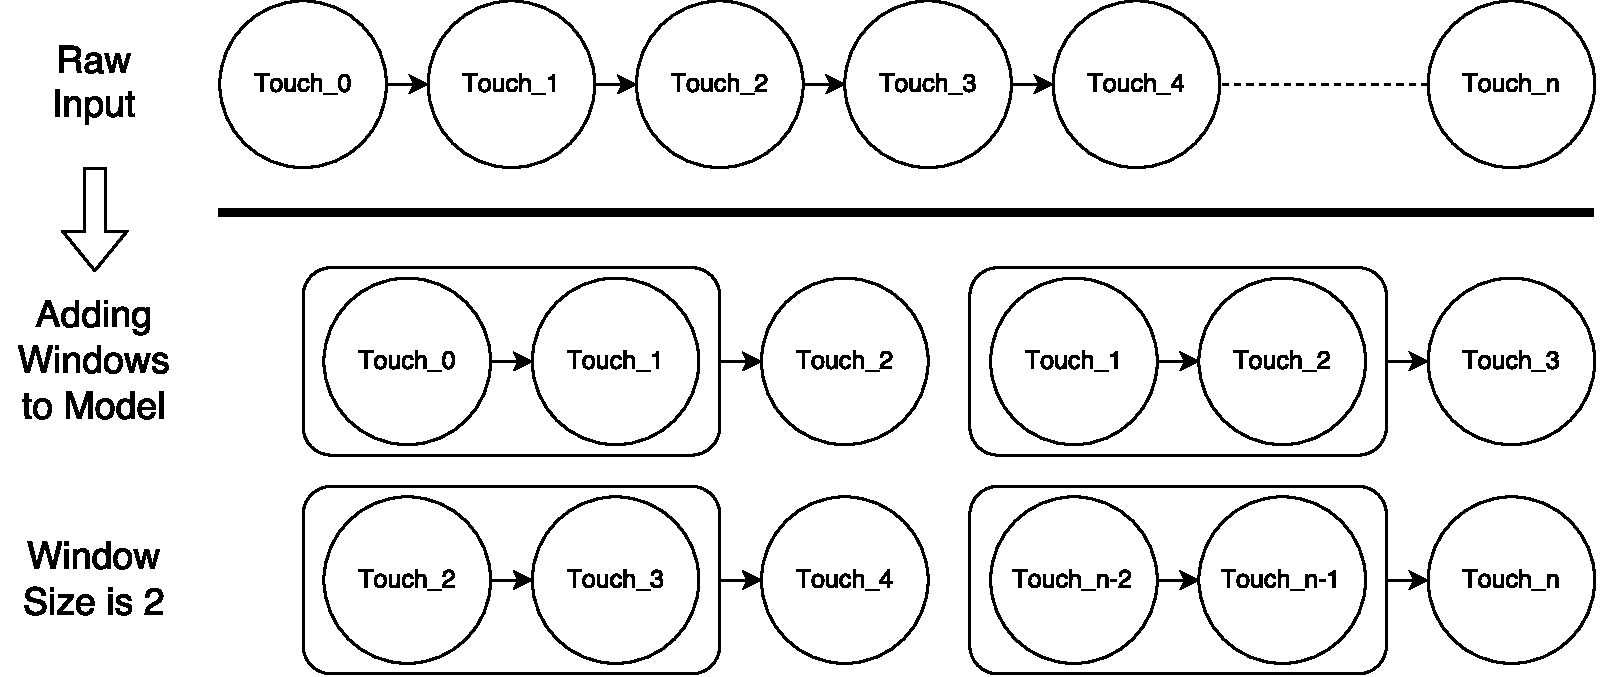
\includegraphics[width=.45\textwidth]{marcov_model_building.pdf}
\caption{
The top of this figure depicts the raw touch screen interaction sequence.
Each touch represents a single interaction between the human user and the soft keyboard.
The diagram's lower portion demonstrates how the raw input is parsed into a 2-Markov model.
The bottom left image can be interpreted to say that Touch\_4 succeeds the sequence Touch\_2, Touch\_3 with some probability $p$.
}
\label{fig:markov_model_building}
\end{figure}

%</markov>

%<*difference>

% describes the difference computation in detail
\begin{figure*}
\centering
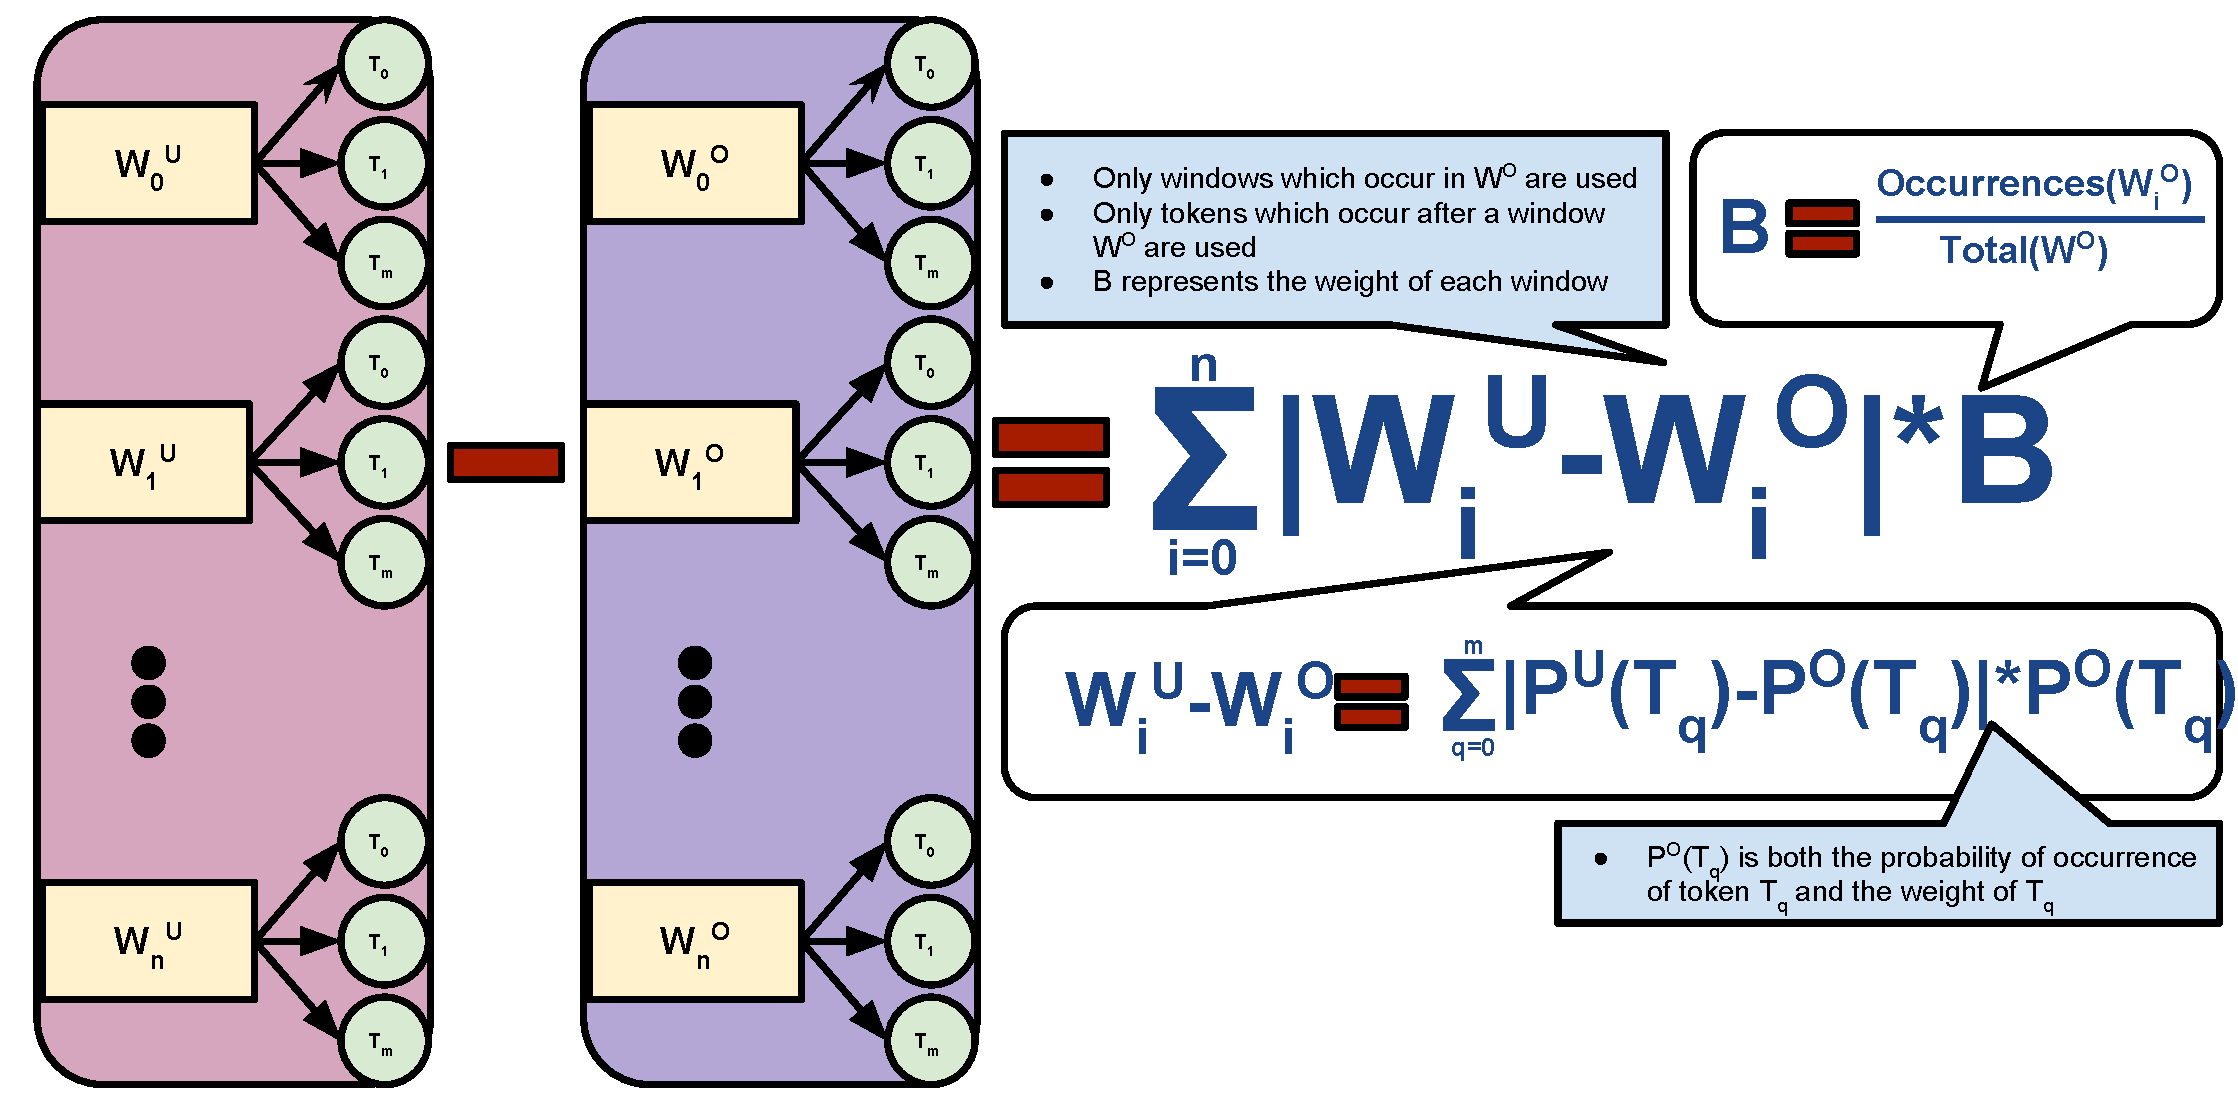
\includegraphics[width=1.0\textwidth]{difference_computation.pdf}
\caption{
Description of the difference metric taken between
$W^U$, the $n-gram$ Markov Model constructed from the authentic user touch screen interactions,
and $W^O$, the $n-gram$ Markkov Model constructed 
from a different set of touch screen interactions.
%
The goal is to determine how closely model $W^O$ is to model $W^U$.
}
\label{fig:difference_computation}
\end{figure*}

%</difference>

%
% details graphics
%

%<*normal>

\begin{figure}
\centering
%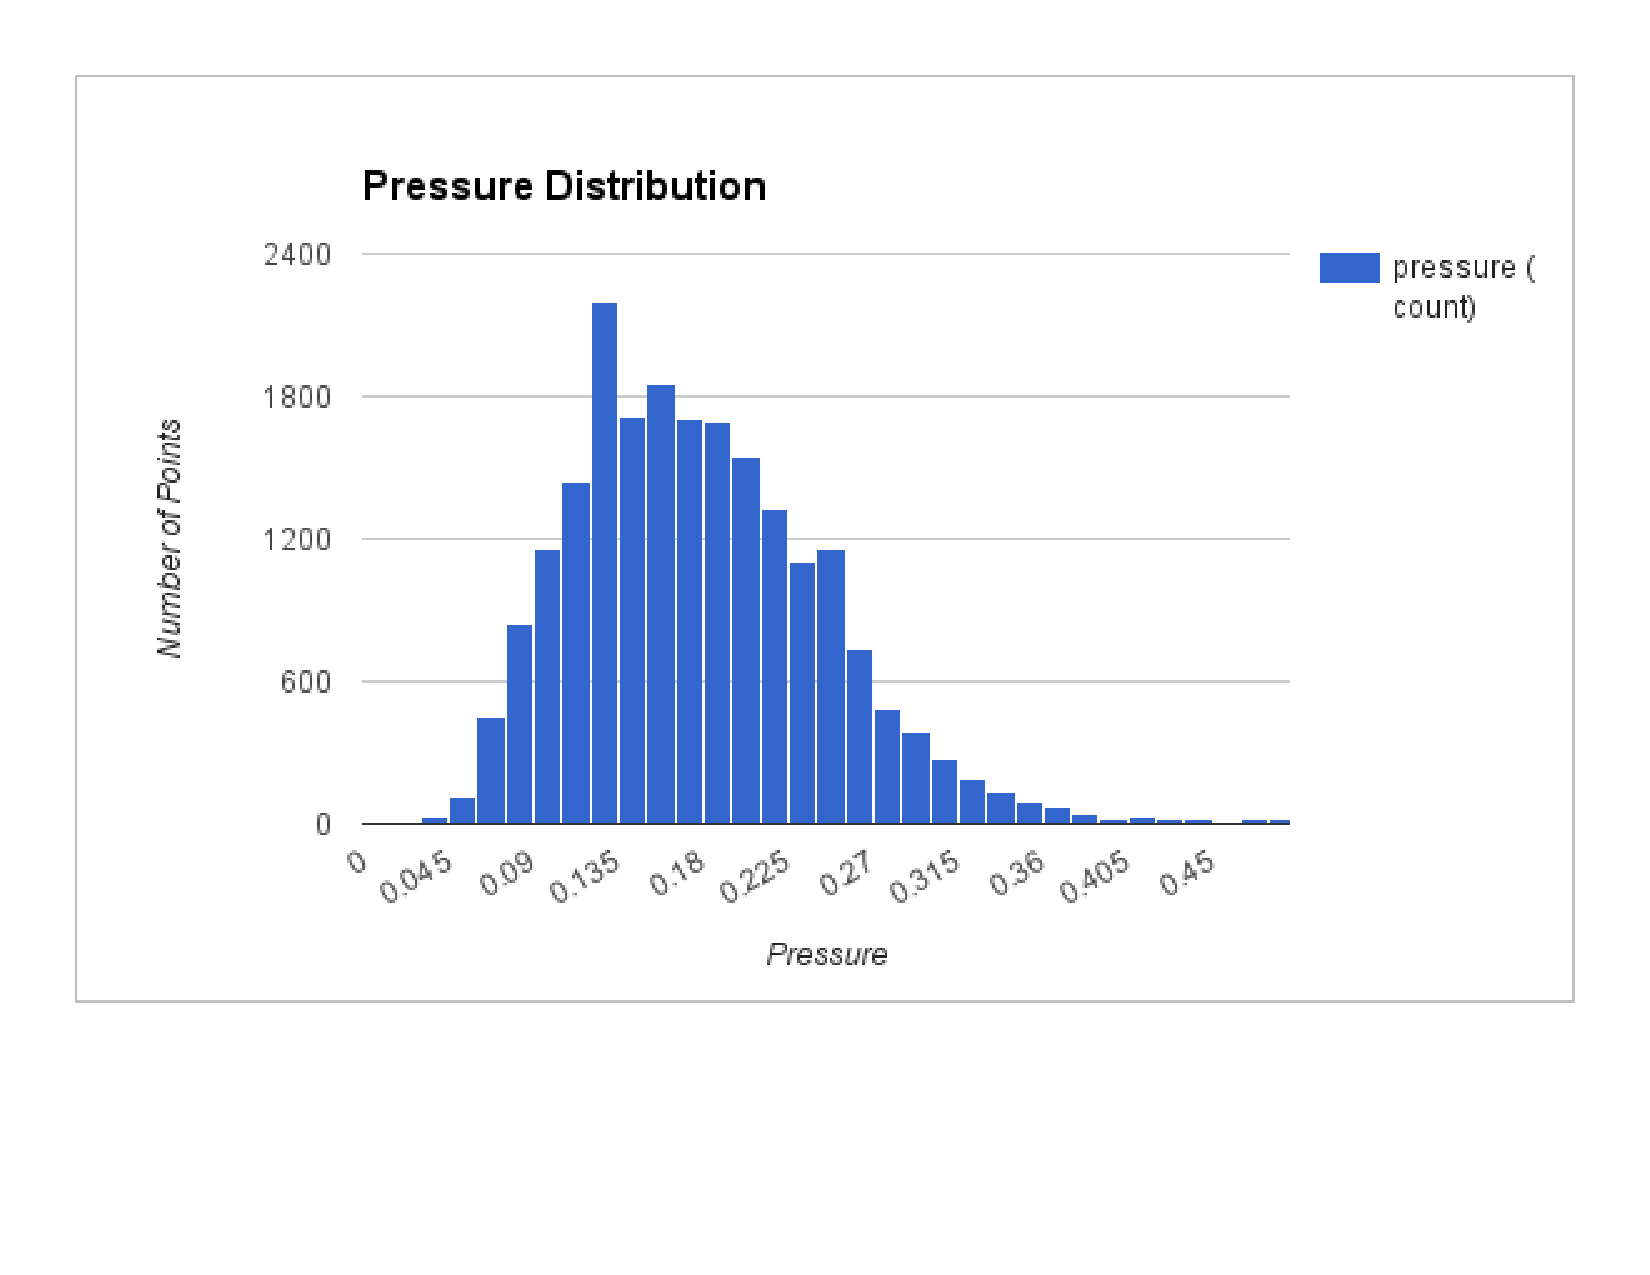
\includegraphics[width=.45\textwidth, keepaspectratio]{pressure_distribution.pdf}
\includegraphics[page=2, width=.45\textwidth, keepaspectratio]{Rplots.pdf}
\caption{
Density of touchscreen interactions' pressure values for one user.
%TODO say what is important about this observation
}
\label{fig:normal_distribution}
\end{figure}

%</normal>

%<*qq>

% shows the qq-plot
\begin{figure}
\centering
%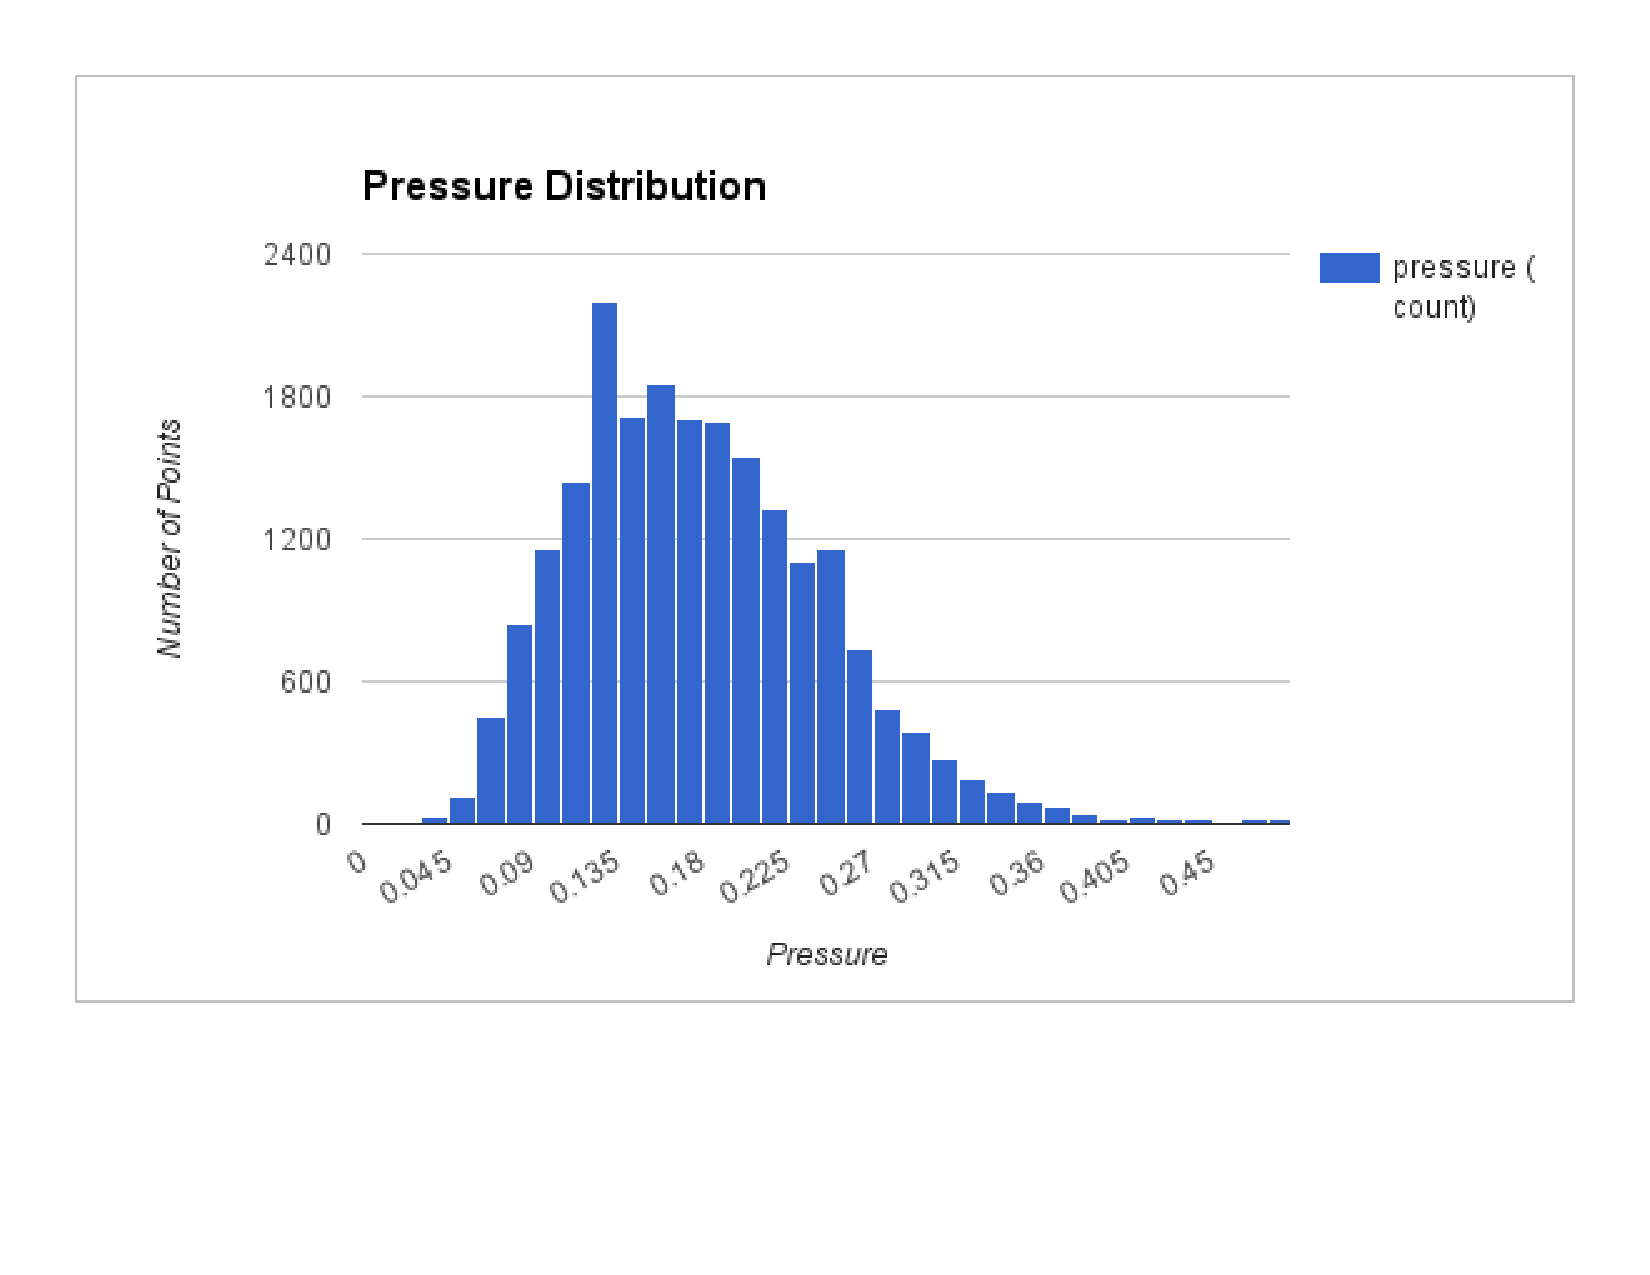
\includegraphics[width=.45\textwidth, keepaspectratio]{pressure_distribution.pdf}
\includegraphics[page=4, width=.45\textwidth, keepaspectratio]{Rplots.pdf}
\caption{
This Q-Q Plot describes data from
a data set having a right skew compared to normally distributed data.
}
\label{fig:qq_plot}
\end{figure}

%</qq>

%<*threshold>

%this figure describes how false positive and false negative percentages vary based on authentication threshold
\begin{figure}
\centering
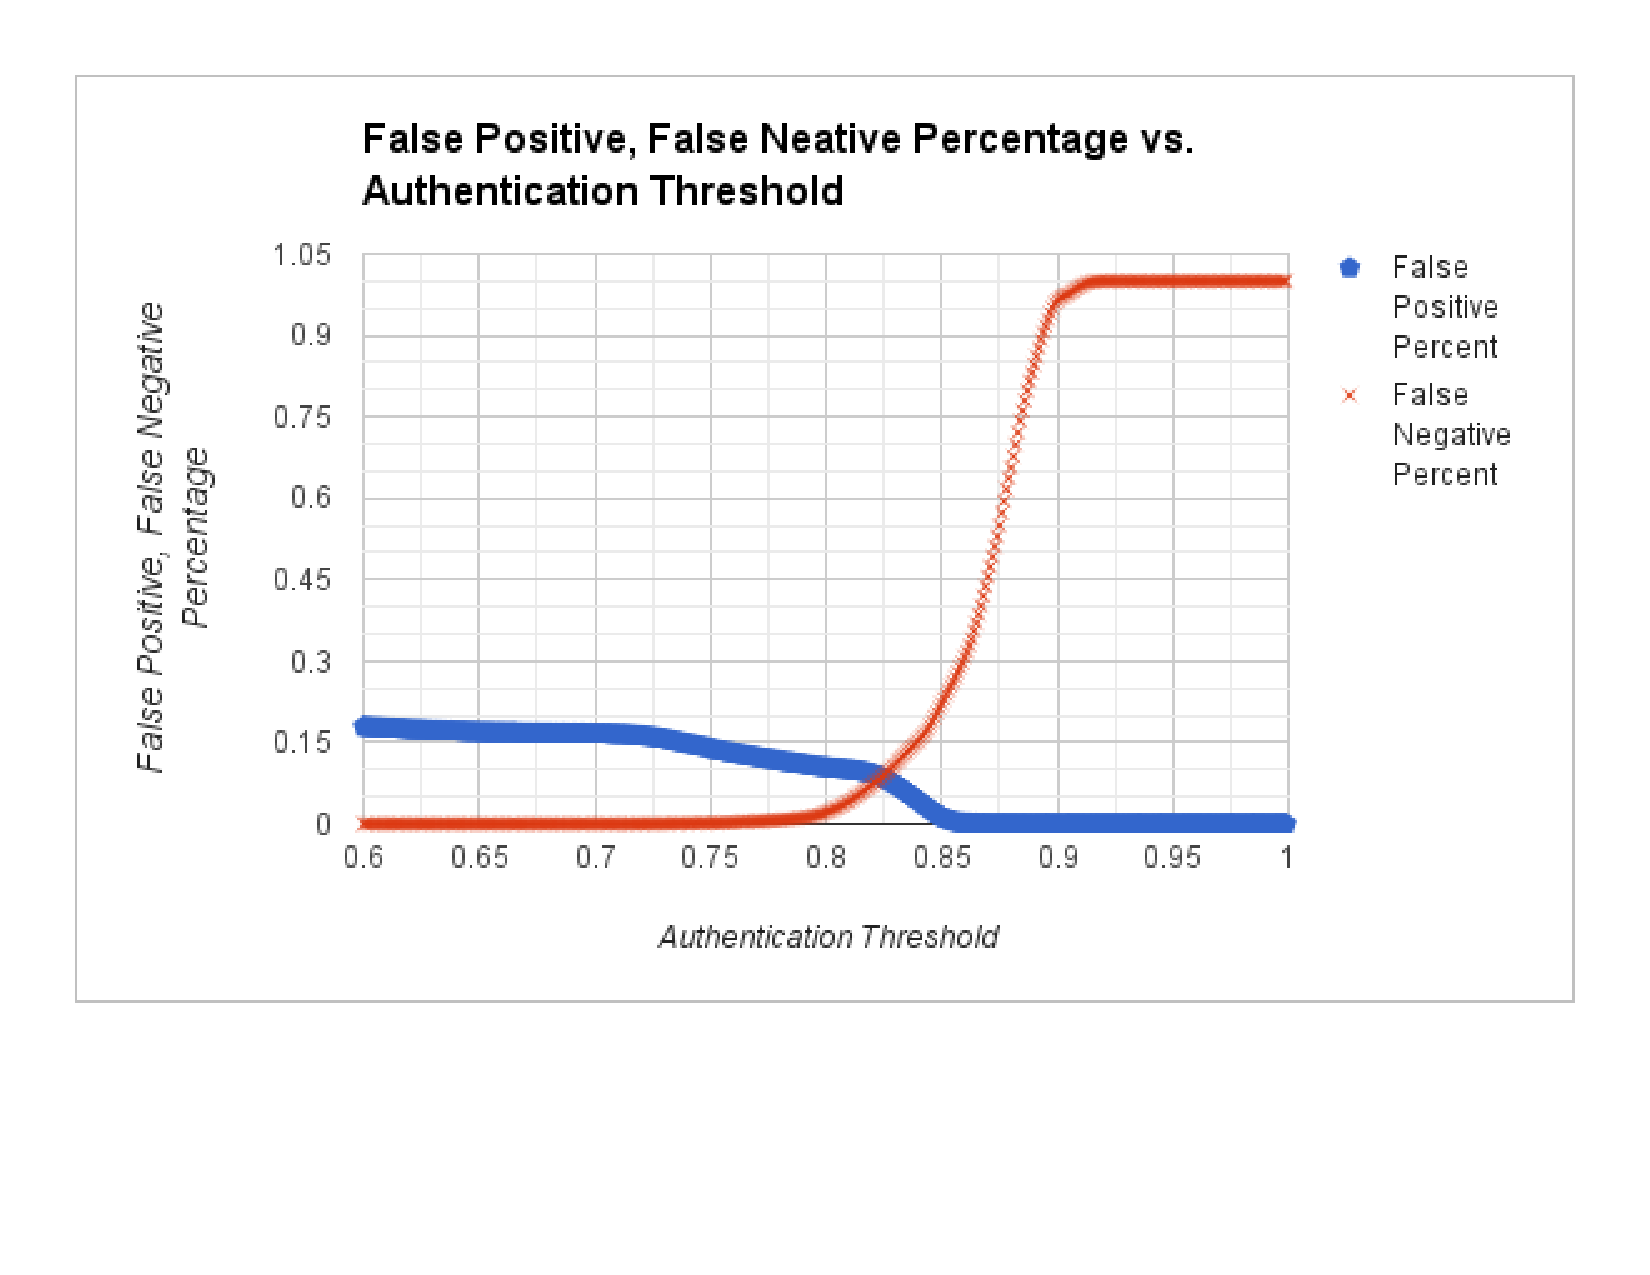
\includegraphics[width=.45\textwidth]{false_positive_vs_authentication_threshold.pdf}
\caption{False positive and false negative percentages vary as the authentication threshold is adjusted.}
\label{fig:threshold_vs_percentages}
\end{figure}

%</threshold>

%<*window>

% this figure describes the effect of window size on authentication accuracy
\begin{figure}
\centering
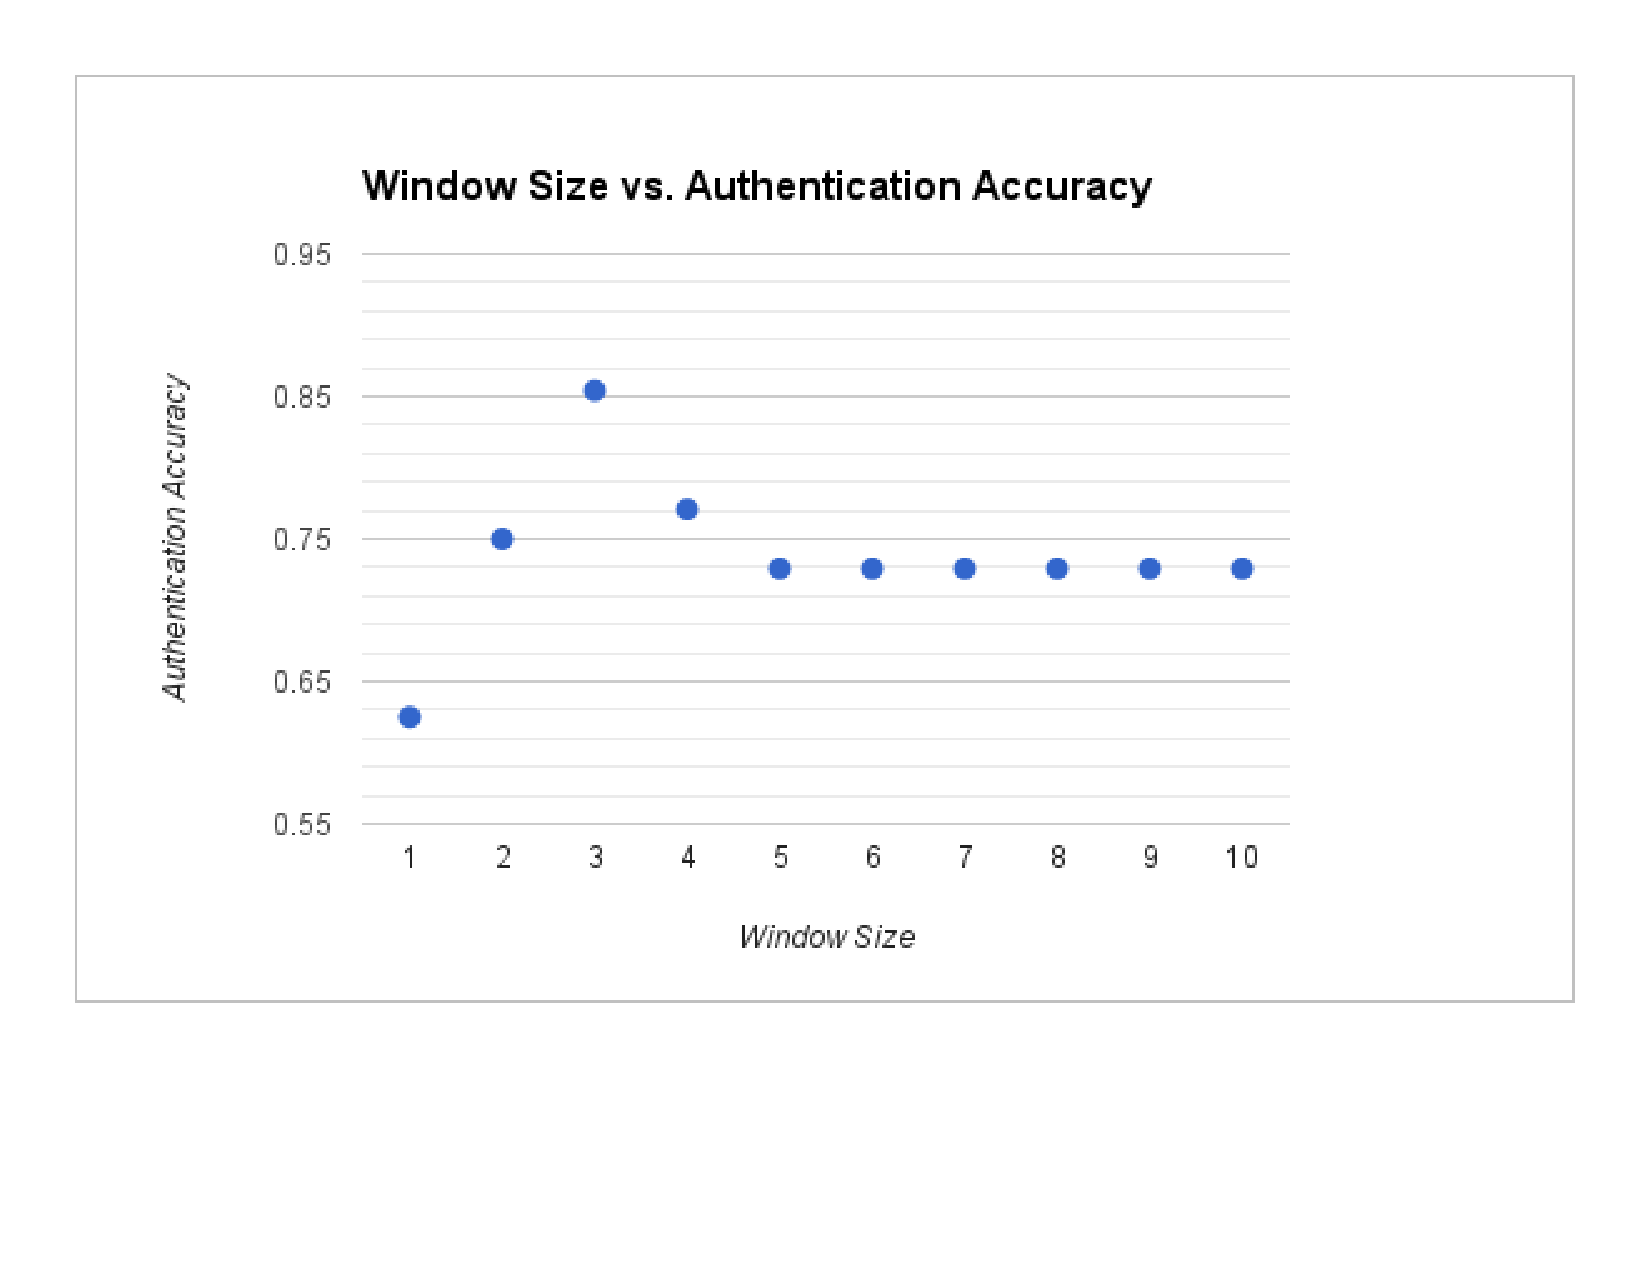
\includegraphics[width=.45\textwidth]{window_size_vs_authentication_accuracy.pdf}
\caption{The effect of $n$ in $n$-Markov Model window size on authentication accuracy.}
\label{fig:window_size_vs_authentication_accuracy}
\end{figure}

%</window>

%<*authentication>

\begin{figure}
\centering
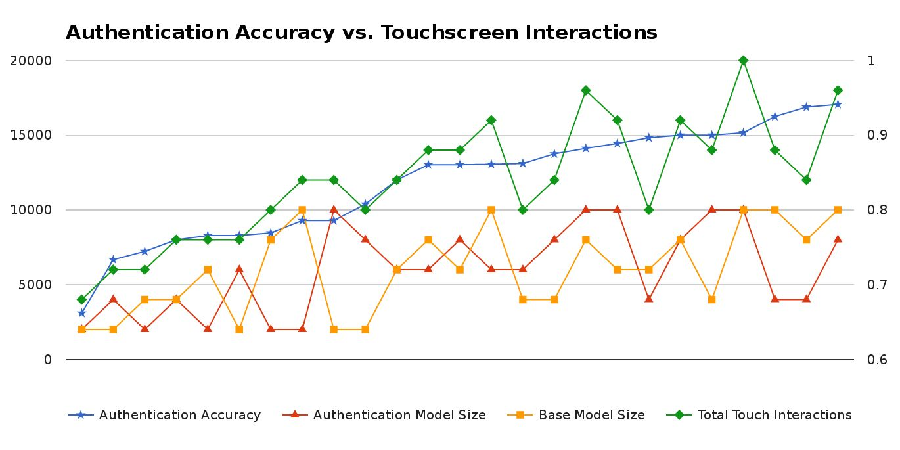
\includegraphics[width=.45\textwidth]{authentication_accuracy_vs_touchscreen_interactions.pdf}
\caption{
The left y axis describes the size of model
in number of touchscreen interactions.
We compare
authentication accuracy(blue star), measured on the right y axis, 
to authentication model size(red triangle),
base model size(yellow square),
and total touch interactions(green diamond)
measured on the left y axis.
Total touch interactions is the sum of
base model size and authentication model size.
}
\label{fig:authentication_accuracy}
\end{figure}

%</authentication>

%<*total>

% describes authentication accuracy dependence on the amount of user data
\begin{figure}
\centering
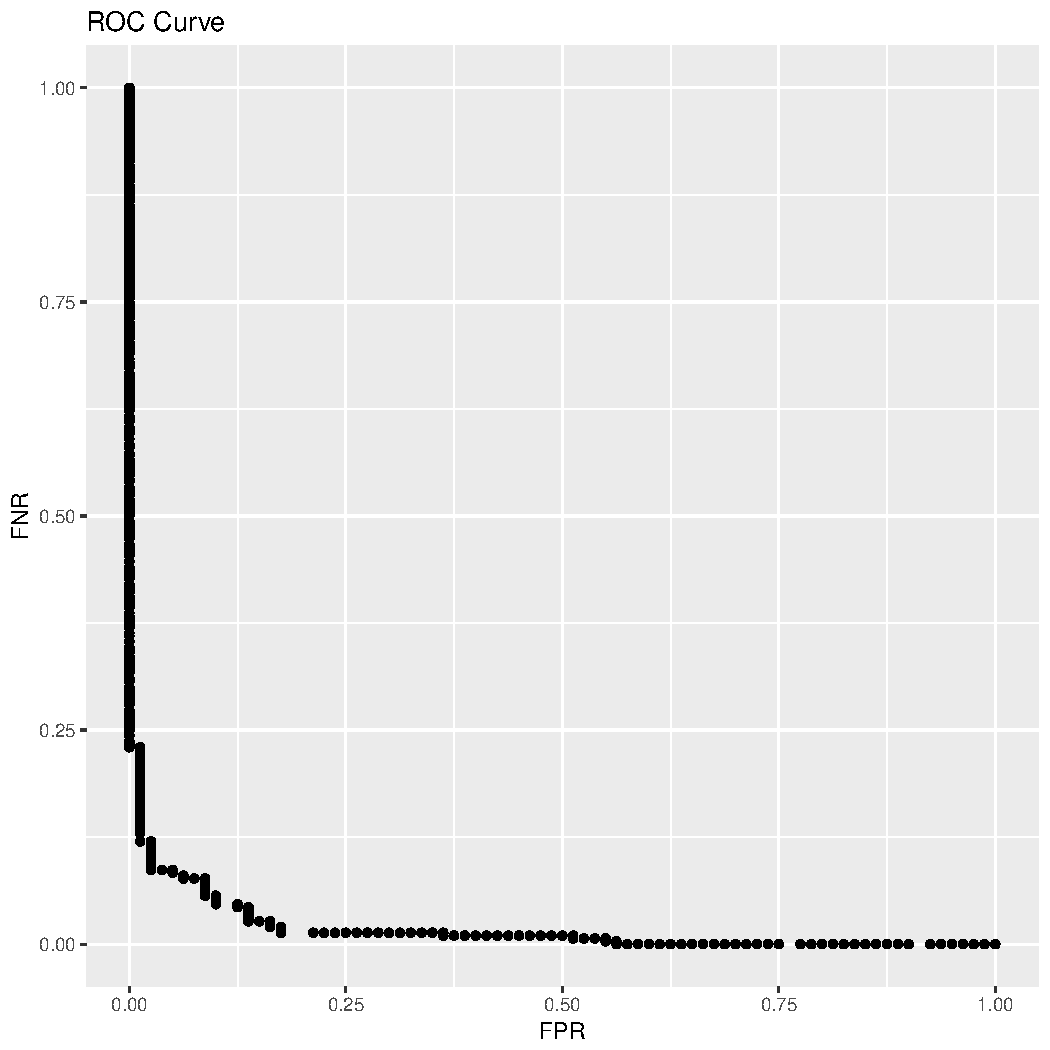
\includegraphics[width=.45\textwidth]{authentication_accuracy_vs_total_interactions.pdf}
\caption{
Authentication accuracy can be seen as 
a function of
the total number of touch screen interactions
used in model construction.
Total touch interactions is the sum of
base model size and authentication model size.
}
\label{fig:total_touches_vs_authentication_accuracy}
\end{figure}

%</total>

%<*nexus>

\begin{figure}
\centering
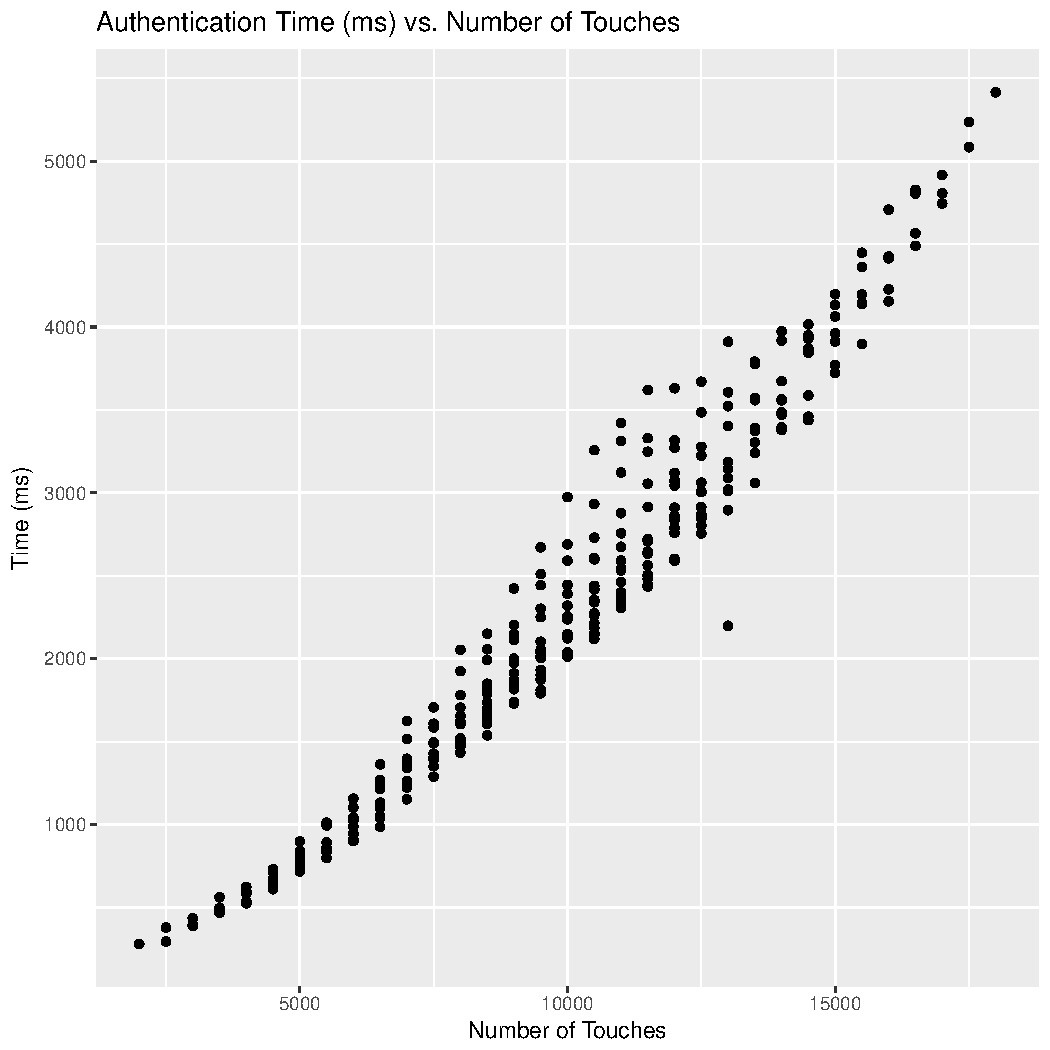
\includegraphics[width=.45\textwidth]{nexus_7_runtimes.pdf}
\caption{
The computation time, measured in seconds(sec), on a Nexus 7 tablet is
a function of
$Total Size =$ {\it base\_model\_size} $+$ {\it auth\_model\_size}.
Model sizes are measured by number of touch interactions used in their construction.
}
\label{fig:nexus_total_size_time}
\end{figure}

%</nexus>
